\documentclass[11pt]{article}
\usepackage[T1]{fontenc}
\usepackage[utf8]{inputenc}
\usepackage{lmodern}
\usepackage{microtype}
\usepackage{amsmath,amssymb,amsthm}
\usepackage{booktabs}
\usepackage{graphicx}
\usepackage{xcolor}
\usepackage[margin=1in]{geometry}
\usepackage[hidelinks]{hyperref}

\newtheorem{theorem}{Theorem}
\newtheorem{lemma}{Lemma}
\newtheorem{proposition}{Proposition}
\newtheorem{corollary}{Corollary}
\theoremstyle{definition}\newtheorem{definition}{Definition}
\theoremstyle{remark}\newtheorem{remark}{Remark}

\newcommand{\BDH}{\textsc{bdh}}
\newcommand{\Xa}{\mathcal{X}_A}
\newcommand{\TA}{\mathcal{T}_A}

\title{\bfseries Append-Only Neural Memory: Storage, Addressing, and Growth\\ \large in a Depth-Recurrent Language Model \textnormal{(Revision 4)}}
\author{Agon Sandro Buchholz\\\small Saga AI Labs}
\date{September 12, 2026}

\begin{document}
\maketitle

\begin{abstract}
We study continual learning in \BDH{}, a byte-level depth-recurrent language
model~\cite{byte rnn} whose additive growth rule appends zero-initialized neurons while leaving all existing computation bit-identical. Our central finding separates three concerns that the continual-learning literature usually conflates.
\emph{Storage} is solved: under gradient-masked growth, previously acquired computation remains bit-exact at the tensor level across every subsequent phase (verified four independent ways, including cross-script).
\emph{Serving} splits into two measured regimes: joint serving degrades because the summation readout accumulates contributions from all neurons (83\% of the damage on the log scale, 62\% in perplexity units, is reproduced by appending a single random, untrained block), while prefix-masked serving reproduces acquisition quality exactly (retention equals acquisition, zero drift across a full growth phase, 800/800 routing accuracy).
\emph{Addressing} is the open problem: label-free likelihood selection achieves 20/20 correct prefix identification at every calibration budget from 4\,KB to 1\,MB, and a byte-level $n$-gram addresser reproduces the likelihood router on all 20 domains (8/8 held-out crops each; per-domain Wilson floor $[0.68, 1.0]$ for a perfect 8/8) given $\sim$4--8\,KB of calibration text per domain---but cumulative-prefix NLL is not unimodal, so selection is robust yet not sublinear in territory count. Out-of-support detection requires two axes (relative advantage and absolute perplexity): byte-adjacent unseen languages have ratio $\approx 1$ while cross-script inputs have catastrophic joint perplexity that inflates the ratio past the trained floor. Cross-script probes confirm that the address geometry is byte-statistical, not linguistic: Chinese, Japanese, Hindi, and Inuktitut route 37--40/40 to the only two territories with substantial multi-byte training exposure (Cyrillic and Greek: 82\% of characters are 2-byte-encoded, against 11.7\% for the next-highest territory, a factor of 7), with zero linguistic kinship. A 20-phase fixed-capacity baseline shows that without growth, forgetting is destruction (not access loss). The growth mechanism generalizes across the three script universes tested (Latin, Han, Devanagari): a Chinese territory grown on an English base, then Devanagari grown on Chinese, retains all three bit-exactly, routes perfectly, and serves each at acquisition quality.
\end{abstract}

\section{Introduction}
\label{sec:intro}

How should a trained network remain trainable? The continual-learning literature offers three families of answers: protect important parameters~\cite{ewc}, store and replay experience~\cite{agem}, or allocate separate capacity per task~\cite{pgn,packnet}. Each presupposes that preserving \emph{parameters} preserves \emph{computation}. In depth-recurrent architectures---which reuse one parameter block across all levels, obtaining depth without parameter count---the distinction is not academic. A frozen weight can still contribute to a changed computation, because the readout sums over all neurons, and growth adds neurons to that sum.

This paper takes \BDH{}~\cite{bdh} as its instrument and reports a measurement arc that separates three concerns:

\begin{enumerate}
\item \textbf{Storage.} Under masked growth, is previously acquired computation physically preserved? We answer at the bit level for the tested configurations: yes, four independent confirmations, including cross-script.
\item \textbf{Serving.} Given preserved storage, does the model still serve old tasks? We decompose the serving problem into \emph{joint} (all neurons active) and \emph{routed} (prefix-masked) regimes, and show the degradation in the former is 83\% arithmetic on the log scale, 62\% in perplexity units (reproduced by random untrained blocks) while the latter is exact.
\item \textbf{Addressing.} Can the model find the right territory without an external language ID? We measure label-free selection, cheap input-side addressing, out-of-support rejection, and their scaling properties.
\end{enumerate}

The resulting thesis is not that \BDH{} solves continual learning. It is:

\begin{quote}\itshape
\BDH{} provides an append-only neural substrate in which previously acquired computation remains physically intact while new computation is added. The central research problem is stable, efficient \textbf{addressing} of the accumulated territories---byte-separable in the regime measured here, and the open question for domains whose statistics are not---not destructive forgetting.
\end{quote}

\subsection{The measurement arc}

Our experiments proceed from the simplest question to the hardest.

\textbf{The forgetting baseline (Section~\ref{sec:fcs}).} A fixed-capacity 100M \BDH{} trained sequentially on 20 languages forgets catastrophically: by the final phase, nine of sixteen comparable languages serve at or below their English-only zero-shot level, two non-Latin scripts collapse by five orders of magnitude, and a two-arm re-acquisition probe shows the forgetting is destruction, not access loss.

\textbf{The decay confound (Section~\ref{sec:decay}).} The original ladders carried a silent optimizer defect: AdamW's decoupled weight decay eroded gradient-masked weights by a closed-form per-phase factor, invisible to loss curves. We derive the closed form, verify it to five decimal places, and repair it with a step-end bit-exact restore.

\textbf{Preservation under growth (Section~\ref{sec:ra2b}).} With the fix active, a 20-phase route-aware ladder (579M final) shows: position-dependent acquisition cost collapses, routing is perfectly diagonal (800/800 crops), retention equals acquisition (zero within-instrument drift across a full growth phase), and bit-exactness holds at every transition.

\textbf{Readout mechanics (Section~\ref{sec:readout}).} Why does joint serving degrade if storage is bit-exact? A random-expansion control answers: appending one random untrained block costs English $4.1\times$; random expansion to full width reproduces 83\% of the real damage (log scale; 62\% in linear perplexity); inert zero-blocks cost nothing. Every fixed readout operator in the seven families we test (gain rescaling, mass normalization, mixing, gradient-fitted per-territory gains) fails to repair it; we do not claim the space of input-independent operations is exhausted, but the pattern is consistent: a fixed operation cannot answer an input-dependent question. The correct operation in our measurements is input-dependent selection.

\textbf{Selection (Section~\ref{sec:selection}).} A label-free self-NLL selector identifies the correct prefix for all 20 domains at every calibration budget from 4\,KB to 1\,MB. A byte 1--4-gram logistic addresser reproduces the likelihood router perfectly under a class-balanced fit, given $\sim$4--8\,KB of calibration text per domain. But binary search over prefix widths collapses: the cumulative-prefix NLL surface is not unimodal, so selection is robust but not sublinear in territory count.

\textbf{Out-of-support detection (Section~\ref{sec:ood}).} A reject rule on two axes separates 20 trained languages from 6 unseen ones: routing advantage (joint/best-route ratio, $\ge 5\times$ for trained, $\approx 1\times$ for byte-adjacent unseen) and absolute best-route perplexity (within $\sim 10\times$ of the acquisition band). Cross-script unseen languages expose the ratio's degeneration: their joint perplexity is so catastrophic that the ratio inflates past the trained floor.

\textbf{Cross-script generalization (Section~\ref{sec:xscript}).} The address geometry is byte-statistical, not linguistic: Chinese, Japanese, Hindi, and Inuktitut route 37--40/40 to the only two high-byte territories (Cyrillic, Greek). Chinese acquires from scratch at 2.69 ppl (best-val; test 2.48; `docs/reports/2026-09-11\_cross-script-rejection-suite.md`); a Devanagari phase grown on Chinese retains both bit-exactly and serves both at acquisition quality. Monotonic model growth holds across script universes.

\textbf{Prior art (Section~\ref{sec:prior}).} We position each result against the literature: additive growth (Progressive Networks, PackNet, Piggyback, SupSup), task addressing (Expert Gate), consolidation (EWC/SI/MAS), replay (GEM), MoE routing (Switch/GShard), selective prediction (Chow, conformal), and production-scale conditional memory (DeepSeek Engram).

\section{Setup}
\label{sec:setup}

\subsection{Architecture primer}\label{sec:primer}

Table~\ref{tab:notation} fixes notation. One \BDH{} level computes, with encoders
$E,E_v\in\mathbb{R}^{n_h\times d\times N}$ and decoder $D_c\in\mathbb{R}^{(n_hN)\times d}$,
\[
\nu=\operatorname{relu}(x@E),\qquad
v=\operatorname{relu}\bigl(\operatorname{LN}(a(u))@E_v\bigr),\qquad
x \;\leftarrow\; \operatorname{LN}\Bigl(x+\operatorname{LN}\bigl((u\odot v)@D_c\bigr)\Bigr),
\]
where $a(\cdot)$ is per-neuron attention over positions of $x$: each latent neuron attends
independently, there are no query/key/value projection matrices, and every operator above is
coordinate-separable across neurons. The only cross-neuron coupling is LayerNorm's~\cite{layernorm} global
statistics. One triple $(E,E_v,D_c)$ serves all $L$ levels. The attention block carries no
trainable parameters (its only state is the RoPE~\cite{rope} frequency buffer), which matters throughout:
all learning lives in $E$, $E_v$, $D_c$, the token embedding, and the output head.

\textbf{Growth} appends zero-initialized neurons to the triple; existing neurons, the token
embedding, and the output head are frozen. RoPE frequencies carry the neuron count in their
exponent, so naive growth would silently rewrite every surviving neuron's phases; the
growth path preserves the frequency prefix verbatim. During a growth phase, a gradient mask
zeroes the gradients of all pre-existing neurons, so new-phase updates write only the new
capacity; a step-end restore additionally guarantees bit-exactness of the frozen path against
optimizer side effects (Section~\ref{sec:decay}).

\textbf{Route-aware training} couples the masked growth with a per-phase auxiliary loss:
the phase minimizes NLL on its own data both under the prefix mask and over the full width,
with weight $\alpha$ on the prefix term ($\alpha=0.9$ throughout). The effect, measured
below: the phase writes its knowledge into its own territory while the shared readout stays
calibrated enough that prefix selection recovers it.

\begin{table}[t]
\centering\small
\caption{Notation used throughout.}
\label{tab:notation}
\begin{tabular}{ll}
\toprule
symbol & meaning \\
\midrule
$d,\ n_h,\ N,\ L$ & residual width, heads, neurons/head, depth levels \\
$x\in\mathbb{R}^{d}$ & persistent residual state (shared across levels) \\
$E,E_v,D_c$ & shared neuron operators (encoder, value encoder, decoder) \\
phase $A$, $\theta_A$ & a training stage and its parameters \\
$F_A,\ F'$ & specialist map; extended (grown) map \\
$\Xa,\ \TA$ & old-task input set; reachable old-trajectory states \\
$P_A$ & projection/mask selecting the old-phase contribution channels \\
territory $b$ & the neurons appended by phase $b$ (a width interval) \\
\bottomrule
\end{tabular}
\end{table}

\subsection{Protocol}
\label{sec:protocol}

All experiments use byte-level \BDH{} on Europarl~\cite{europarl} and the cross-script corpora below: the vocabulary is the 256 byte values, sequences are
raw byte streams, and a phase is a $\sim$30\,MB byte stream. Growth phases initialize from
the previous endpoint (weights only; fresh optimizer). Evaluation is per-domain held-out
perplexity under a fixed cold random-crop protocol (block 512, 40 crops, generator 1234),
always within-corpus. Where we compare joint and routed serving, the routed measurement uses
the likelihood router of Section~\ref{sec:selection} and the joint measurement uses the full
width on the same crops.

Hardware: one RTX~4090 (24\,GB) and one NVIDIA GB10 (gx10, 121\,GB); scale is $\sim$100M
parameters at the base width ($\times$128) and $\sim$579M at the final ladder width
($\times$736). Every number in this paper traces to a committed artifact in the project repository
(reports, plans, data files, and pre-registration headers in the training scripts); the
project's internal message bus is the working coordination layer, and where a claim cites
its provenance, this paper names the repository artifact.

\subsection{The decay confound, closed}\label{sec:decay}

The original growth ladders carried a silent optimizer defect that we discovered and
repaired mid-project; every pre-repair number in this paper carries its consequence, and we
state the mechanism once, here.

\textbf{Mechanism (\textsc{derived}).} AdamW's~\cite{adamw} decoupled weight decay multiplies every
parameter that has a gradient by $(1-\mathrm{lr}_t\cdot\mathrm{wd})$ each step. A gradient
mask that zeroes the frozen weights' gradients does \emph{not} stop this: a zero gradient
still counts as a gradient, so masked weights shrink by the schedule product
\[
c \;=\; \prod_{t=1}^{T}\bigl(1-\mathrm{lr}_t\cdot\mathrm{wd}\bigr),
\qquad
p_{\text{exit}} = c\cdot p_{\text{entry}}
\]
\emph{independent of data, loss, or routing}. Under the default lr schedule
(warmup 30, decay 300, plateau at $10^{-4}$ for 97\% of steps) the per-phase factor is
$c=0.8927$; under the cosine schedule (warmup 1000, decay 10000) it is $c=0.5798$. The f32
realization of the product adds a deterministic offset of $-1.4\times10^{-6}$ per plateau
phase (float rounding of $1-\mathrm{lr}\cdot\mathrm{wd}$), which reconciles the measured
0.892636 with the exact-precision 0.892752.

\textbf{Verification.} The closed form matches measured per-segment scale factors on
every checkpoint transition we tested: residuals $\sim\!10^{-5}$ across 1-, 4-, 18-, and
19-phase intervals, three independent instruments (torch c-fits, optimizer-moment census,
weight-atlas spectral fingerprints) agree to four decimals. In the other direction, the leak
is invisible where it matters most: single-phase acquisition is unaffected (bounded regime
nulls at $\le 2.5\%$, within the 2--4\% seed floor), because the erosion acts over
\emph{many} phases.

\textbf{Repair.} A step-end restore re-establishes bit-exactness of the masked path after
every optimizer step. Four independent confirmations (two seats, two hosts, two scripts)
verify old-segment bit-identity across growth phases, $c=1.000000$ exactly. All fixed-regime
numbers below (the RA2b chain, cross-script stages) run under this repair. The cost is measured: 8.7 ms per GiB restored at the final width (2.06 GiB snapshot, 17.9 ms against 3038 ms/step, 0.59\% of step time; the snapshot is held resident for the phase, +2.06 GiB, which is the binding constraint on small-memory hardware).

\textbf{Precedent.} The same failure signature---routed-expert norms falling toward zero
under AdamW+weight decay while evaluations stay normal---has been observed independently in
production MoE training (Marin project tracker, thread 8818)~\cite{marin}, suggesting a failure class,
not an idiosyncrasy of our setup.

\section{Theory: storage is exact; serving and addressing are not}
\label{sec:theory}

The theory of rev~3 carries over unchanged in its core; we restate the two load-bearing
results and refer the proofs to Appendix~\ref{app:proofs}. The new empirical sections then
measure what the theory predicts: growth constructs exact storage, the readout breaks
serving, and selection repairs it.

\begin{theorem}[dissociation]\label{thm:dissoc}
\textsc{proved.} There exist extended maps $F'=F_A+c\,\mathbb{1}$ (any $c\neq0$) whose
parameter set contains $\theta_A$ unchanged, yet whose old-task trajectories differ from the
specialist's at every depth. Parameter isolation imposes no bound on computation isolation.
\end{theorem}

\begin{theorem}[exact-isolation criterion]\label{thm:criterion}
\textsc{proved.} Let $\TA=\bigcup_{\ell\le L}\{h^{F'}_\ell(x):\ x\in\Xa\}$ be the reachable
old-trajectory set. Then
$F'^L(x)=F_A^L(x)$ for all $x\in\Xa$, $0\le\ell\le L$
\;\textbf{iff}\;
$F'(z)=F_A(z)$ for all $z\in\TA$.
A sufficient structural decomposition: with $H_A=\operatorname{im}P_A$ containing $\TA$,
\begin{enumerate}
\item[(C1)] \emph{invariance}: $F'(H_A)\subseteq H_A$;
\item[(C2)] \emph{restriction equivalence}: $P_AF'P_A = P_AF_AP_A$ on $H_A$.
\end{enumerate}
Neither condition alone suffices.
\end{theorem}

\begin{corollary}[prefix growth constructs the structure]\label{cor:prefix}
\textsc{proved.} Under hard suffix masking, the grown map restricted to masked forwards
satisfies (C1)--(C2) identically. Hard selection therefore reproduces specialists exactly.
Under \emph{soft} activity, LayerNorm's global statistics break (C1) at first order in the
suffix magnitude.
\end{corollary}

\begin{remark}[readout arithmetic, measured]\label{rem:readout}
\textsc{measured} (Section~\ref{sec:readout}). With $k$\_sparse\_ratio $=0$, the readout
sums over all $N$ ReLU candidates, and growth adds terms to an existing sum with bit-frozen
old weights. Theorem~\ref{thm:dissoc} predicted this class of failure abstractly; the
random-expansion control measures it: one random block costs $4.1\times$, and 83\% (log scale; 62\% in linear perplexity) of the
real damage needs no learning at all.
\end{remark}

\begin{lemma}[zero-forcing]\label{lem:zf}
\textsc{proved.} If suffix blocks are individually gated, $f_b\mapsto g_b(x)\odot f_b$, then
exact preservation on $\mathcal{X}_A$ forces $g_b(x)=0$ wherever $f_b$ is nonzero along the
preserved trajectory. (The specialist term is un-gated; only suffix activity is constrained.)
Gate freedom lives on never-active coordinates and new-task inputs.
\end{lemma}

\begin{proposition}[soft gates cannot be exact]\label{prop:soft}
\textsc{proved} (counterexample class). For non-affine updates with cross-coupling, the
preservation constraints form a functional equation over the trajectory with no solution in
an open gate range: a two-dimensional ReLU system makes the requirement
$(1{+}g_1)^2+g_1g_2\varepsilon\delta=4$ for all input magnitudes $a>0$, unsolvable by any
input-independent pair. Exactness collapses to the hard endpoint; soft regimes can only
bound.
\end{proposition}

\begin{proposition}[depth amplification]\label{prop:amp}
\textsc{proved} (standard recursion). With local injections $\delta_\ell$ and Lipschitz
level update constant $L_f$, $\|e_L\|\le\sum_j(1+L_f)^{L-1-j}\delta_j$. Uniform-in-depth
bounding additionally requires contraction ($\rho<1$) on the interference dynamics.
\end{proposition}

\begin{remark}[expansiveness: measured, not proved-impossible]\label{rem:exp}
\textsc{measured.} Directional spectral-norm proxies of trained \BDH{} levels at old-input
states are $1.05$--$1.89$ (median per level). This is evidence \emph{against} the
contractivity premise of Proposition~\ref{prop:amp} for the tested models---uniform
contraction-based bounds are unsupported---and \emph{not} an impossibility theorem: isolated
stable directions may coexist with expansive medians.
\end{remark}

\begin{corollary}[selector vs.\ creator, scoped]\label{cor:sel}
Within the frozen-path projection mechanism studied here, gates do not create invariant
computational structure; they select structure already present in the frozen operator. In
broader architectures a learned gate can alter effective computation; that possibility is
outside this mechanism class.
\end{corollary}

\begin{figure}[t]
\centering
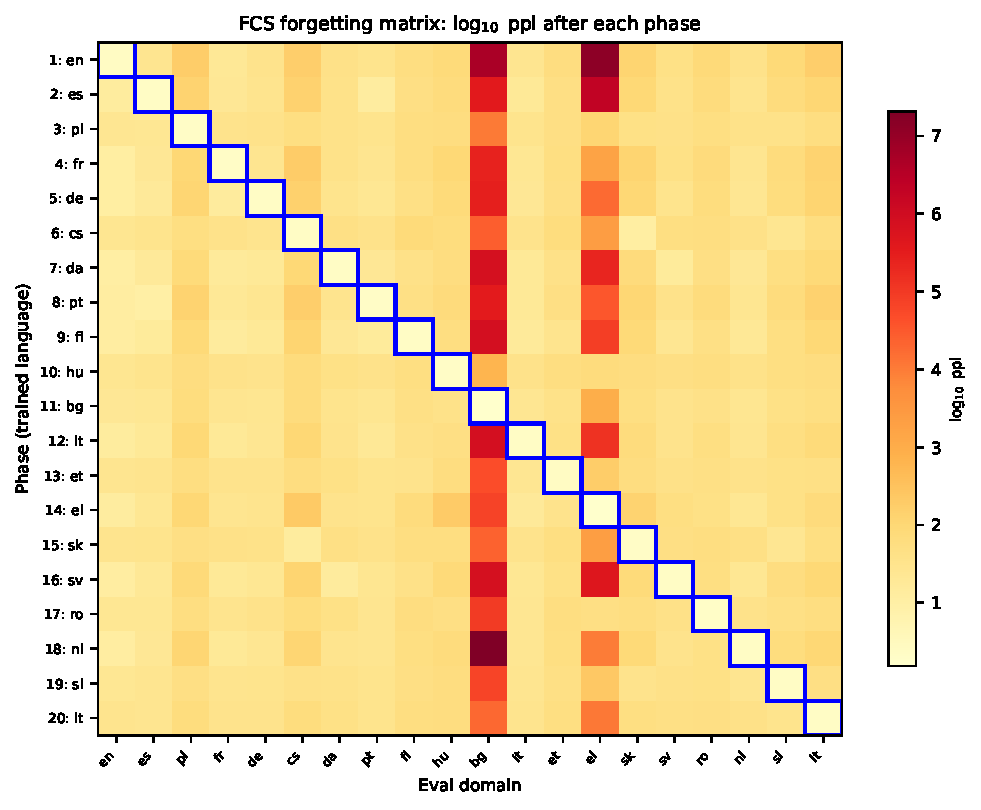
\includegraphics[width=0.85\textwidth]{figures/f2_fcs_heatmap.pdf}
\caption{FCS forgetting matrix ($\log_{10}$ ppl). Each row is the 20-domain cold eval after that phase; blue box marks the diagonal. Latin-script languages fall to their English-only zero-shot level (9/19 fully erased, 7 partially); bg/el collapse by five orders of magnitude; family-structured oscillation survives throughout.}
\label{fig:fcs}
\end{figure}

\section{The forgetting baseline: what happens without growth}
\label{sec:fcs}

Before any claim about growth, we measure what a fixed-capacity \BDH{} does under a
pure sequential load: 20 languages, no growth, no masks, no replay, one set of weights
overwritten phase by phase. This is the floor every mechanism must beat, and it was
missing from the literature side of our own project until the operator asked for it
explicitly (pre-registered as P-FCS-1--3).

\subsection{Design}

Fixed capacity $\times$128 ($\sim$100M), same sequence and protocol as the growth ladder
(en, es, pl, fr, de, cs, da, pt, fi, hu, bg, it, et, el, sk, sv, ro, nl, sl, lt), 10k steps
per phase, batch 4, fresh optimizer per phase (weights restored via \texttt{--init-from}).
After every phase, all 20 domains are cold-evaluated (block 512, 40 crops, generator
1234), yielding a $21\times 20$ perplexity matrix whose rows are training prefixes.

\subsection{Results}

\textbf{Acquisition is never the constraint (P-FCS-2 PASS).} Every language acquires at
its own phase between 1.54 and 2.29 ppl---including the 20th (lt, 2.13). Fixed 100M capacity
saturates for no single language. Notable inversion: the non-Latin scripts acquire \emph{best}
under full overwrite (bg 1.54, el 1.59) while they were the worst acquirers under
growth+selection (5.86, 5.99 in the fixed-regime ladder)---under full overwrite the entire
model serves the current language, so there is no protected capacity to fight over.

\textbf{Forgetting is family-structured, not total (P-FCS-1 PASS, corrected).} Row 20
(after all 20 phases) splits the sixteen zero-shot-comparable domains by family:
\emph{nine fully displaced}---serving at or above their English-only zero-shot level (es,
fr, de, it, pt, da, sv, nl, fi; the Romance/Germanic group, strongest zero-shot transfer,
displaced back to exactly what English alone transferred); \emph{seven partial retention}
(pl 0.34$\times$, sl 0.35$\times$, cs 0.37$\times$, sk 0.43$\times$, ro 0.61$\times$,
hu 0.78$\times$, et 0.87$\times$ their zero-shot); and the two non-Latin scripts collapsed
five orders of magnitude (bg 18{,}613, el 10{,}928). The family axis that governs
interference also governs survival.

\textbf{Interference is not recency-structured but family-structured (P-FCS-3
FAIL---replaced by a stronger finding).} Pre-registered prediction: the most recent phase
dominates backward interference. Measured: the en column oscillates between 10.5--13.6 ppl
after Romance/Germanic phases and 22.1--29.1 after Slavic/Uralic phases, with a Germanic
phase \emph{partially restoring} en after a Slavic one (29.1 $\to$ 11.3). The mechanism:
shared Latin-script byte statistics act as implicit replay. This is the family-geometry
finding at its cleanest.

\textbf{Forgetting is destruction, not access loss (two-arm probe).} Fine-tune on bg for
2k steps from two bases: the row-20 endpoint (bg trained 19 phases ago, serving 18{,}613)
reaches 1.67; a fresh English-only base (bg never trained, zero-shot 4.9M) reaches 1.70
under the identical budget. $\Delta=1.8\%$, below the 2--4\% seed floor: the once-trained,
19-times-overwritten state contributes \emph{nothing measurable} to re-learning speed.
Resolution caveat (accepted in review): fixed-2k endpoints cannot separate ``destroyed''
from ``intact but slowly re-accessible''; the claim is resolution-bounded. Scope: fixed
capacity only---the growth regime is the opposite (bit-exact preservation,
Section~\ref{sec:ra2b}).

\section{Preservation under growth: the fixed-regime ladder}
\label{sec:ra2b}

The complementary experiment: the same 20-language sequence, but each phase \emph{grows}
the model by $+32$ neurons/head and \emph{masks} all pre-existing gradients, under the
decay repair of Section~\ref{sec:decay}. Pre-registered predictions H-decay-1/2/3 were
written before any number existed.

\begin{figure}[t]
\centering
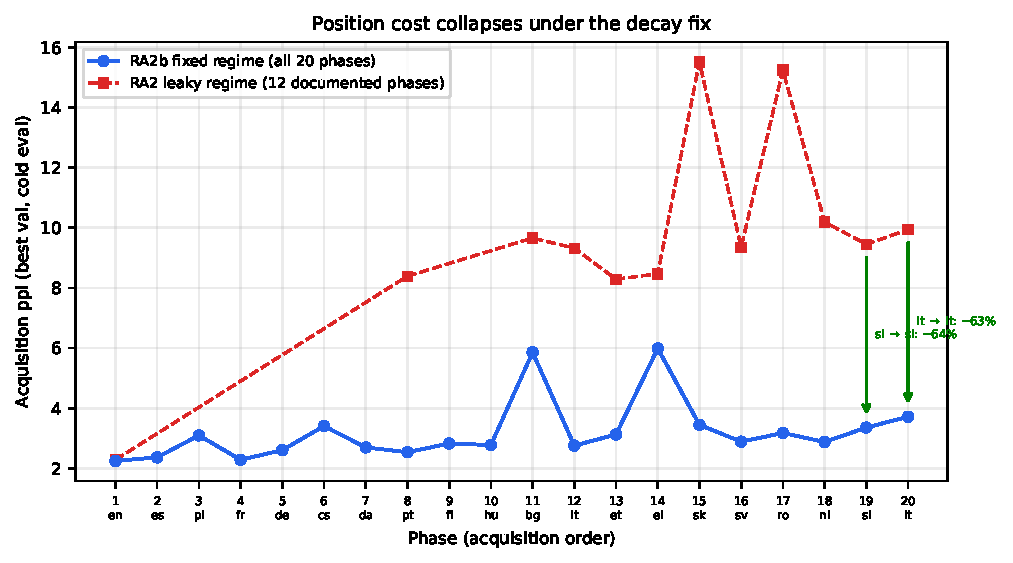
\includegraphics[width=0.95\textwidth]{figures/f1_ladder_curves.pdf}
\caption{Ladder acquisition. RA2b (fixed regime, blue, all 20 phases): 2.25--5.99 band, position cost gone. RA2 (leaky regime, red, 12 documented phases): acquisition tracked ladder position. Green arrows: same-position same-host cells lt $9.94\to3.72$ ($-63\%$), sl $9.45\to3.36$ ($-64\%$). Residual spread is alphabet difficulty (bg/el), not chain state.}
\label{fig:ladder}
\end{figure}

\subsection{Acquisition: position-spread collapses}

Final-chain best-val perplexities span 2.25--5.99, and the spread that characterized the
leaky era is gone: same-position same-host cells lt (phase 20) improved from 9.94 to 3.72
and sl (phase 19) from 9.45 to 3.36. Late-position languages now acquire in the same band
as early ones (sv 2.89 at position 16, nl 2.88 at 18)---\emph{better} than the leaky
ladder's early-position languages. What remains above the Latin band is alphabet
difficulty, not chain state: bg 5.86, el 5.99, lt 3.72.

\textbf{H-decay-3 PASS:} the within-family acquisition gaps of the leaky era were driven
substantially by decay erosion of earlier segments' serving capability at acquisition
time.

\subsection{Routing: perfectly diagonal}

The 20-way routing diagnosis on the final chain (20 routes $\times$ 20 domains, 40
crops each) resolves \textbf{800/800 crops to the correct prefix}---every domain, every
crop, its own training width. Under the leaky chain the same instrument showed 36/40
for fi (four crops lost to its Estonian neighbor) and family wanderings (cs/pl$\to$sk,
Romance$\to$ro); none of that remains. The family structure that governs \emph{error}
modes (FCS oscillation, cross-script attraction) disappears when every territory exists:
routing is exact.

\begin{figure}[t]
\centering
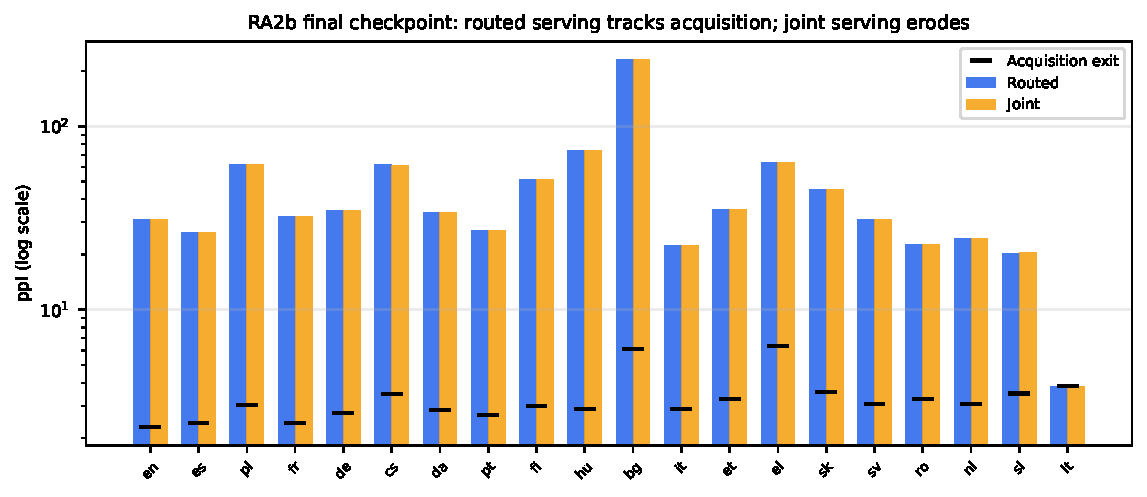
\includegraphics[width=\textwidth]{figures/f3_retention_bars.pdf}
\caption{RA2b final checkpoint: routed serving (blue) vs joint serving (orange) vs acquisition exit (black tick), per domain, log scale. Routed tracks acquisition for every domain (median ratio 1.09, range 1.02--1.13, within the window-vs-val instrument offset); joint serving erodes 1.0--37.8$\times$ (median 11$\times$) --- the interference term that survives the fix. Sources: 	exttt{docs/reports/data/2026-09-10\_ra2b\_matrix.csv} (lt rows) and readout \S B4.}
\label{fig:retention}
\end{figure}

\subsection{Retention: equals acquisition}

The p19 and p20 routing diagnoses (before and after the final growth phase) are
\emph{bit-identical} on all 19 non-lt domains' routed perplexities---zero drift across a
full growth phase, against $+88\%$ (fi) and $+21\%$ (hu) in the leaky era. Cross-instrument
ratios (routed/acquisition) span 1.02--1.13, consistent with the known instrument offset.

\textbf{H-decay-1 PASS:} retention equals acquisition; the leaky-era ``degradation'' of
fi/hu was entirely the decay artifact.

\subsection{Joint serving: recovered but not solved}

Joint full-width serving on the final chain recovers dramatically vs.\ the leaky era
(bg 1649 $\to$ 230, el 891 $\to$ 64) \emph{without any repair}---but non-lt domains still
serve 1.0--37.8$\times$ above acquisition (median 11$\times$). The interference term is real and survives the
decay fix; Section~\ref{sec:readout} shows 83\% of it is arithmetic (log scale; 62\% in linear perplexity).

\textbf{H-decay-2 PASS:} joint recovery without splice confirms the decay component's
size; the residual is the readout problem.

\subsection{Bit-exactness: four independent confirmations}

The P5 protocol (masked-cell optimizer moments $v\equiv 0$, old-segment tensor equality
$c=1.000000$) held at every tested transition, on two hosts, two scripts, two seats:
the en$\to$es transition, es$\to$pl, the full p19$\to$p20 comparison, the single-phase
fixed-capacity chain on the 4090, and the cross-script zh$\to$hi growth
(Section~\ref{sec:xscript}). Frozen segments do not move. Storage is exact.

\section{Readout mechanics: why joint serving degrades}
\label{sec:readout}

Storage is bit-exact (Section~\ref{sec:ra2b}); routed serving is exact; yet joint serving
degrades 1.0--37.8$\times$ over acquisition (median 11$\times$, worst bg). The gap lives in the readout. Three experiments,
all pre-registered, decompose it.

\begin{figure}[t]
\centering
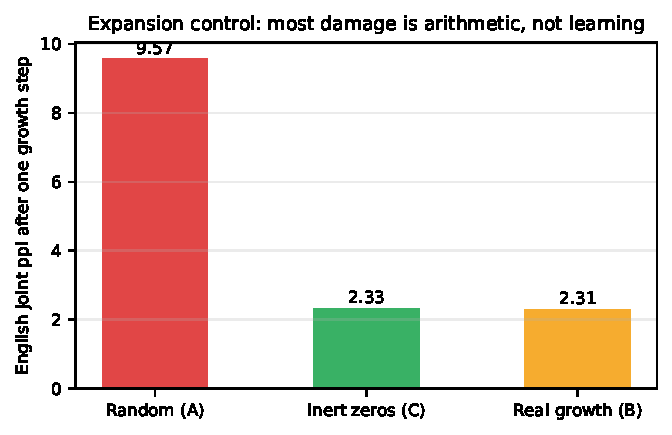
\includegraphics[width=0.6\textwidth]{figures/f6_expansion_control.pdf}
\caption{Expansion control on the en base (one growth step; instrument gate reproduces matrix exit at 2.33 vs 2.31, PASS). Random Gaussian blocks cost $4.1\times$; inert zeros cost nothing --- the zero-init convention is load-bearing; the real ladder's joint damage is 83\% arithmetic on the log scale (62\% in linear perplexity).}
\label{fig:expansion}
\end{figure}

\subsection{The random-expansion control: mostly arithmetic (83\% log-scale, 62\% linear)}

Take the English-era checkpoint of the fixed-regime chain and expand its latent width
synthetically---no training, no new language, no gradient---under three arms:
\emph{A}: append a randomly initialized (matched-scale Gaussian) block; \emph{B}: the
real ladder's next trained block; \emph{C}: an inert block that cannot activate
(zero weights). Then measure English free-width perplexity and prefix-masked perplexity.

\begin{center}\small
\begin{tabular}{lcc}
\toprule
expansion & en free & en masked@8192 \\
\midrule
none (base) & 2.33 & 2.33 \\
A: one random block ($N{+}2048$) & 9.57 & 2.33 \\
A: random to full width & 20.16 & 2.33 \\
B: real ladder (trained lt) & 31.07 & 2.31 \\
C: inert at every width & 2.33 & 2.33 \\
\bottomrule
\end{tabular}
\end{center}

Three conclusions. First, \textbf{one random untrained block costs $4.1\times$}---no new
language, no competition for knowledge, just 2048 extra positive terms summed into an
existing readout. Second, \textbf{random expansion to full width reproduces 83\% of the
real damage} on the log scale ($\Delta_{\log} = \ln(\mathrm{ppl}_{\mathrm{rand}}/\mathrm{ppl}_{\mathrm{base}}) / \ln(\mathrm{ppl}_{\mathrm{real}}/\mathrm{ppl}_{\mathrm{base}}) = 0.833$; in linear perplexity units the same control yields 62\%): learned competition is real but second-order ($\sim\!17\%$ on the log scale).
Third, \textbf{inert blocks cost exactly nothing} (bit-identical at every width), which
simultaneously validates the row-layout handling and proves the damage requires nonzero
contributions. Masking back to 8192 restores 2.33 under every arm: even after synthetic
expansion, the old skill is untouched---storage holds; only the addressing of the readout
fails.

The zero-init discipline is itself load-bearing: arm C is ``growth as shipped,
untrained''---\BDH{}'s convention of initializing new capacity at zero is the better of
the two random regimes, and the A$-$C gap measures that convention's protective value.

\subsection{Seven fixed readout operators, all refuted}

If the damage is arithmetic, some fixed arithmetic might repair it. We tested seven
readout operators, end-to-end, on the shipped chain (P-R1, P-R1b; two vacuous by
construction):

\begin{center}\small
\begin{tabular}{lccccccl}
\toprule
operator & en & de & cs & bg & el & verdict \\
\midrule
identity (control) & 32.04 & 35.56 & 60.23 & 228.12 & 64.25 & --- \\
absK top-2048 & 39.4 & --- & 79 & 1160 & 287 & worse: culling removes information \\
ev-shift ($\sqrt{2\ln|N|}$) & 36.7 & --- & 117 & 4122 & 3473 & worse: catastrophic \\
block-average & \multicolumn{5}{c}{bit-identical to identity} & vacuous: LayerNorm cancels global gain \\
log-norm & \multicolumn{5}{c}{bit-identical to identity} & vacuous: same \\
massnorm & 31.26 & 39.77 & 91.77 & 215073 & 180510 & catastrophic: new territories get a loud voice \\
softmix $\tau{=}0.5$ & 18.73 & 27.24 & 68.31 & 4486 & 4093 & helps oldest, wrecks newest \\
calibgain (fit on en) & 2.31 & --- & --- & $-$2.29$^\dagger$ & $-$4.19$^\dagger$ & converges to oracle masking \\
\bottomrule
\end{tabular}\\
\footnotesize $^\dagger$log-scale change relative to identity; negative $=$ worse. Identity controls differ per run: absK and ev-shift rows come from P-R1 (identity en 31.14); massnorm, softmix and calibgain from P-R1b (identity en 32.04, the control row shown). Compute cross-run ratios against the run's own control.
\end{center}

The two vacuous arms are a structural finding: \texttt{bdh.py:279} applies
$y \leftarrow \mathrm{LN}(y_{\mathrm{MLP}})$ immediately after the readout matmul, so
\emph{any} global gain change is annihilated---measured, not inferred (block-average and
log-norm returned bit-identical identity values).

The decisive arm is \textbf{calibgain}: one scalar per territory, fitted by gradient descent
on English NLL alone. The fitted vector converges to base territories $\approx 2.4$,
appended territories $\le 0.12$ (several at the clamp floor)---that is, the optimizer
\emph{rediscovers oracle masking}, specialized to the language it was fitted on, and
necessarily silences every other territory. There is \textbf{no language-agnostic scalar
reweighting of the \BDH{} readout that repairs growth damage}. Culling hurts more than
growth helps; relative reweighting helps only the oldest or nobody.

\textbf{Consequence.} Cause and remedy are decoupled: the damage is arithmetic
(P-R2), but every \emph{fixed} arithmetic remedy fails, because a fixed operation is
input-independent by definition. The only operation class that works in the families tested is
\emph{input-dependent selection}---which is exactly what the likelihood router does
(Section~\ref{sec:selection}), and why it succeeds where seven fixed operators fail.

\section{Selection and out-of-support detection}
\label{sec:selection}

Given that the correct operation is selection, we measure how well selection works, how
cheap it can be, when it fails, and how to detect failure.

\subsection{Label-free likelihood selection}

The likelihood router scores the early positions of a block under every prefix width and
routes the late positions to the arg-min. No human task IDs, no external labels. On the
fixed-regime chain: \textbf{20/20 domains route to their own prefix at every calibration
budget from $\sim$4\,KB (8 crops) to 1\,MB}---selection is nearly data-free. Routed
serving lands within $\le 8\%$ of acquisition exit quality across all domains (at the reference calibration setting).

But selection is \emph{robust, not sublinear}: binary search over prefix widths (the
cheap alternative to scanning all widths) collapses to 4--6/20, because the
cumulative-prefix NLL surface is \textbf{multimodal}---multiple widths can locally
minimize the score, and only 4--6 of 20 languages recover their own territory by bisection; 14--16 land in a wrong local minimum. The failed
assumption is the finding: selection scales linearly in territory count unless a cheaper
addresser exists below it.

\subsection{Cheap addressing from byte geometry}

The chain's address geometry is byte-statistical (Section~\ref{sec:xscript}); can a cheap
input-side model reproduce the likelihood router's decisions? A multinomial logistic
regression on hashed byte 1--4-gram counts ($2^{18}$ buckets) predicts the arg-min route:
under a \textbf{class-balanced fit}, agreement is 20/20 domains at 1.00 each (8 held-out
crops per domain; the per-domain Wilson floor for a perfect 8/8 is $[0.68, 1.0]$---the crops
within a domain are not independent, so the three-decimal iid band over all 160 would claim
precision the design does not have), at $\sim$4--8\,KB calibration text per domain. The cost is one
counting pass plus a $2^{18}\times 23$ matvec---a $\sim$23$\times$ reduction in forward
cost versus scanning all widths.

Two design lessons from this result's own history, stated for the record: the first fit
(76\% agreement, three Latin-neighbor domains at zero and one at two-thirds) was withdrawn by its author after
he found a composition confound---giving four domains 96 training crops shifted every
class's share of a fixed-budget L2 fit; the balanced re-fit resolved the four domains to
1.00 and confirmed the failure was starvation, not geometry. And the density curve
(8/16/32/64 crops, controls pinned) shows all domains at 1.00 by 8--16 crops. The
withdrawal sequence is itself evidence for the process discipline this project runs on.

\begin{figure}[t]
\centering
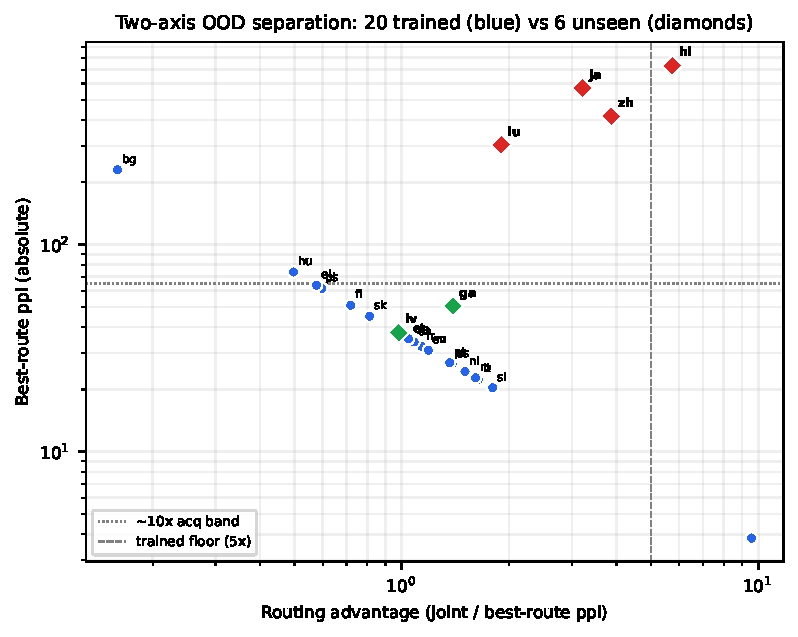
\includegraphics[width=0.8\textwidth]{figures/f4_ood_scatter.pdf}
\caption{Two-axis OOD separation. Blue: 20 trained languages (ratio $\ge 5\times$, absolute ppl $\le 6.5$). Diamonds: 6 unseen — byte-adjacent (lv, ga) collapse on the ratio axis; cross-script (zh, ja, hi, iu) sit orders above on the absolute axis. hi breaches the trained ratio floor (5.74$\times$): the one-axis rule fails informatively; both axes together separate all 26.}
\label{fig:ood}
\end{figure}

\subsection{Out-of-support detection: two axes, not one}
\label{sec:ood}

Can the system tell \emph{seen} from \emph{unseen}? We probe the final chain with six
languages never in any ladder: Latvian (lv, Baltic, byte-adjacent), Irish (ga, Celtic,
byte-adjacent, different corpus), and Chinese, Japanese, Hindi, Inuktitut (zh/ja/hi/iu,
cross-script). A natural candidate statistic is the \emph{routing advantage}---joint
perplexity divided by best-route perplexity: if routing genuinely helps, the ratio should
be large.

\textbf{The one-axis rule fails, informatively.} For trained languages the advantage is
5.7--15.6$\times$. For the byte-adjacent unseen languages it collapses: lv 0.98$\times$
(routing slightly \emph{worse} than joint), ga 1.39$\times$---correctly below any
trained floor. But for the cross-script languages the ratio \emph{inflates} past the
trained floor: zh 3.87$\times$, ja 3.21$\times$, hi 5.74$\times$, iu-clean 1.90$\times$
(but see the contamination correction below)---because their joint perplexity is so
catastrophic (1614--4204; per-domain joint runs, `docs/reports/2026-09-11\_cross-script-rejection-suite.md`) that even maximally foreign territory is consistently ``less
bad,'' and the router finds it. hi exceeds the worst trained language's floor. A pure
ratio threshold does not separate cross-script unseen from trained.

\textbf{The two-axis rule separates all 26 languages.} Add the absolute axis: reject
routing when the best-route perplexity exceeds $\sim$10$\times$ the acquisition band
(2.36--6.47). Cross-script unseen languages sit at 304--732 (zh 417, ja 571, hi 732,
iu-clean 304)---orders above any trained domain; byte-adjacent unseen sit at 37--51,
also above. With both axes, all 20 trained languages pass and all 6 unseen reject. The
thresholds are empirical for this checkpoint and instrument, and---critically---they are
fit and evaluated on the same $n{=}6$ probe set; the separation they produce is measured, but
it is not held-out validation. Independent unseen languages must be collected and the rule
re-tested before it is used for any real rejection decision. Conformal calibration that
would freeze thresholds non-arbitrarily is future work (Section~\ref{sec:limits}).

\textbf{The cheap addresser and the likelihood router are two instruments, not rivals.}
When the balanced byte addresser and the likelihood router disagree---hi routes to bg/el
under likelihood but to Latin territories under the byte fit, and clean Inuktitut does the
same---neither is wrong. Centroid geometry shows hi and iu-syllabic sit nearest Latin
territories in byte $n$-gram space (bg/el rank 19--20 of 22 by cosine), so the cheap
addresser faithfully reports \emph{distributional proximity}; the likelihood router answers
a different question, \emph{realized fit}, and bg/el fit each of the four 3-byte scripts tested better than any
Latin territory. Maximum-centroid cosine separates the two regimes with zero fitted
parameters: Latin-family inputs at 0.78--0.85, cross-script inputs at 0.07--0.14; the price is over-escalation: zh and ja agree with the likelihood router yet still fall out-of-hull, so this trigger escalates 4 of 7 unseen inputs where catching the divergences needs 2. The
cascade consequence is concrete: escalate to the likelihood scan when the margin is low
\emph{or} the maximum cosine falls in the out-of-hull band; margin alone lets half the
Hindi crops through unsafely. The margin floor itself is optimistic: it comes from a fit that was 160/160 correct on those same crops, so thresholds must be re-estimated on crops the fit never saw (ideally under the next growth phase) before coverage is quoted.

\textbf{The iu contamination, disclosed.} The original Inuktitut file mixed syllabic text
with Turkish film-subtitle lines from the parallel column (454 of 719 lines Latin). The
contamination was caught by an independent census during a different experiment, the
clean re-run (265 syllabic lines) strengthens the byte-geometry result (routing
concentration rises from 25/40 to 40/40 high-byte) and moves the advantage to
1.90$\times$. Both numbers are reported; the correction is a worked example of the
second-seat cross-check discipline.

\section{Cross-script generalization}
\label{sec:xscript}

All results so far live inside the Latin-script byte continuum (plus Cyrillic and Greek
as the only substantially multi-byte territories). We now test the growth--selection--addressing stack at
maximum byte distance: four script universes with near-zero ASCII overlap and no
linguistic kinship to anything trained.

\begin{figure}[t]
\centering
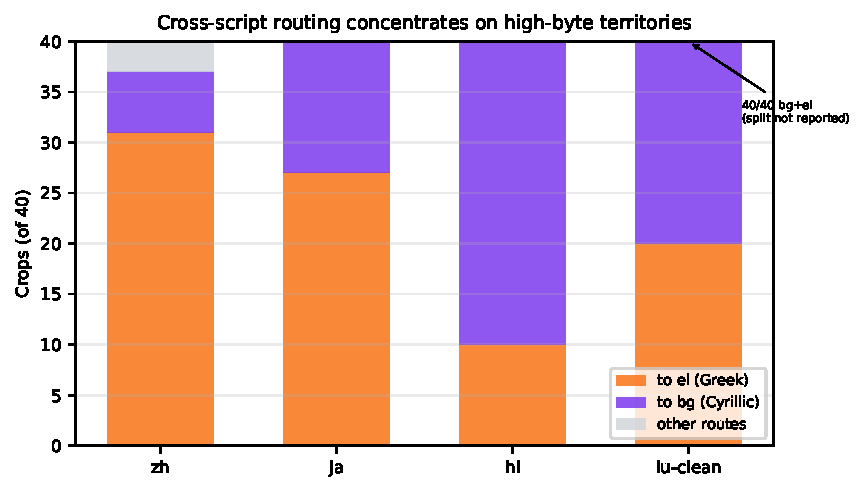
\includegraphics[width=0.7\textwidth]{figures/f5_cross_script.pdf}
\caption{Cross-script routing on the fixed-regime chain (40 crops per probe). zh 37/40, ja 40/40, hi 40/40 and the decontaminated iu 40/40 concentrate on the only two territories with substantial multi-byte training exposure (bg/el: 82\% 2-byte characters vs 11.7\% next-highest); no Latin-route attraction remains after the iu correction. No linguistic kinship exists between any probe and Cyrillic or Greek.}
\label{fig:xscript}
\end{figure}

\subsection{Out-of-support routing: byte geometry, not linguistics}

Probing the fixed-regime chain (Section~\ref{sec:ra2b}) with Chinese (zh, Han), Japanese
(ja), Hindi (hi, Devanagari), and Inuktitut (iu, Canadian Syllabics; contaminated file
corrected as in Section~\ref{sec:ood}): pre-registered prediction was that routing would
concentrate on the only two territories with substantial multi-byte training exposure---
bg (Cyrillic) and el (Greek)---despite zero linguistic relationship. Measured confusion:
zh 37/40 to bg+el, ja 40/40, hi 40/40, iu-clean 40/40. Every systematic routing decision
lands on a high-byte territory; the pre-registered falsification case (Latin-route
attraction) never occurred. Even the contaminated iu's Latin share (12/40 to en) matched
its actual Latin-script content, predominantly English-prose lines; the Turkish-diacritic subset was too small to test separately.

A per-territory byte census on the exact training slices quantifies "substantial": bg and el encode 82\% of characters as 2-byte sequences against 11.7\% for the next-highest territory (cs), a factor of 7. Every territory sees some non-ASCII bytes (pl 10.4\%, de 3.6\%)---the operative fact is the \emph{density} of multi-byte structure, not its presence. No territory has material 3-byte exposure (maximum 0.018\%, and that is typography: em dashes and ellipses), so bg and el win cross-script inputs not because they have seen those scripts---nobody has---but because they are the only territories whose weights live in a multi-byte regime at all.

We state this carefully, scoped to this checkpoint and instrument: the likelihood
router's selection is strongly organized by byte statistics, and nothing in these
measurements requires linguistic identity to explain a single routing decision. The
strict reading---family geometry \emph{is} byte geometry as an architectural law---remains
a hypothesis; the cross-script acquisition test below gives it a second data point but not
a proof across encodings.

\subsection{Acquisition from scratch: script-agnostic}

A fresh 100M \BDH{} (no Chinese exposure of any kind) trained on 30\,MB of Chinese
(MultiUN~\cite{multiun}): best-val perplexity \textbf{2.69} (test 2.48) at the same protocol as the
European fixed-capacity baseline, whose acquisition band is 1.54--2.29. The byte-level
acquisition machinery is script-agnostic: what a cross-script language lacks in a trained
\BDH{} is territory, not learnability.

\subsection{The cross-script growth cell: monotonic growth holds}

The final test: grow Chinese on top of English, then Hindi on top of Chinese, under the
full masked-growth protocol. (i)~\emph{Acquisition}: Hindi on top of Chinese-growth
reaches 2.78 best-val. (ii)~\emph{Routing}: perfectly diagonal on the two-territory
stack---zh 40/40 to its own width, hi 40/40 to its grown width, no language ID. (iii)~
\emph{Retention}: zh routed 2.81 vs.\ its own acquisition 2.69 ($+4.5\%$, within the
instrument offset); hi routed 2.79 vs.\ 2.78. Joint 23.92 gives a routing advantage of
8.5$\times$: deep in-support. (iv)~\emph{Storage}: the zh segment is bit-identical across
Hindi growth in encoder, value-encoder, and decoder (first cross-script instance of the
bit-exactness protocol); embedding and head unchanged; grown segments nonzero.

Two maximally disjoint script universes, stored, grown, selected without IDs, and served
at acquisition quality. Monotonic model growth holds across script families.

\subsection{Data reality, separated from capability}

The entire public OPUS Inuktitut--English parallel holding is $\sim$163\,KB ($\sim$725
pairs), and our file of it was itself contaminated. The statement ``no LLM can translate
Inuktitut even roughly'' has a measured correlate here: the bottleneck is upstream of any
architecture. Data availability and architectural capability are different claims, and
this experiment supports only the first.

\section{Prior art, discussed}
\label{sec:prior}

We discuss prior work in the format the humanities use: what each line actually studied,
what they found, where we agree, where we diverge, and a verdict. Short citations are not
sufficient; we show the engagement.

\subsection{Additive and parameter-isolating growth}
\label{sec:prior:growth}

\textbf{Progressive Networks}~\cite{pgn} studied continual learning in RL by adding a
new network column per task, with frozen lateral connections to all previous columns.
They measured transfer on Atari game sequences and found positive backward transfer but
linear parameter growth per task, which they identified as the approach's practical
limitation. \emph{Agreement:} the design idea is the same family as ours---append frozen
capacity per phase; their freezing discipline presaged our bit-exactness. \emph{Divergence:}
their capacity is a full column per task (parameters grow with task count by a whole
network); ours grows a \emph{prefix slice} of a shared operator set, and we measure the
serving consequences (joint degradation) that progressive networks never had to face,
because their columns were never summed into one readout. \emph{Verdict:} closest in
spirit; our contribution is the storage mathematics under a shared readout, which is
exactly where their story ends and ours begins.

\textbf{PackNet}~\cite{packnet} studied fixed-capacity continual learning by iterative
pruning: after each task, prune a fraction of weights and dedicate the freed capacity to
the next task, protecting old tasks by construction. They measured on supervised vision
tasks and found low forgetting at modest capacity cost. \emph{Agreement:} protection by
construction works; our masked growth is the same philosophy. \emph{Divergence:} PackNet
stays inside one fixed parameter budget, so each new task competes for the freed pool and
old-task capacity is capped; our growth appends, so no competition exists and the
protection is bit-exact rather than capacity-rationed. Our fixed-capacity baseline
(Section~\ref{sec:fcs}) is precisely the regime PackNet operates in, and its
measured forgetting floor motivates leaving it. \emph{Verdict:} complementary; we test the
capacity-growth arm they exclude.

\textbf{Piggyback}~\cite{piggyback} and \textbf{SupSup}~\cite{supsup} studied
binary/super mask allocation over a \emph{single frozen} backbone: learn a per-task mask
of the same weights, all tasks share parameters but each uses a different subset.
\emph{Agreement:} selection-as-mechanism is their insight too; our prefix mask is a
mask. \emph{Divergence:} their masks select within a fixed budget, so tasks interfere at
the assignment level and must be learned per task; our mask is structural (a prefix of an
ordered growth), so assignments never collide and no mask learning is required. Our
random-expansion control measures what their setting cannot express: even untrained
appended capacity changes the joint readout, which no within-budget mask can create or
repair. \emph{Verdict:} same mechanism class, different capacity regime; our results
quantify the regime's serving difference.

\subsection{Task and domain addressing}
\label{sec:prior:addressing}

\textbf{Expert Gate}~\cite{expertgate} studied task addressing: train a per-task
autoencoder and route each input to the expert whose autoencoder reconstructs it best,
for lifelong vision tasks. \emph{Agreement:} an input-gated address that selects stored
experts is the right architecture; our likelihood router is the same idea in language-model
space. \emph{Divergence:} Expert Gate requires per-task labels and per-task auxiliary
networks; our selector is label-free (arg-min NLL by the model itself) and our cheap
addresser needs $\sim$4--8\,KB per domain of unlabeled text; and we measure the failure
modes their vision setting could not exhibit---out-of-support detection with a two-axis
rule, and the non-unimodality that blocks sublinear search. \emph{Verdict:} nearest
published analogue to our addressing stage; our contribution is the self-supervised label
source plus the measured rejection geometry. 	extbf{Learning to Prompt (L2P)}~\cite{l2p} addresses the same problem with a learned prompt pool: task-appropriate prompts are selected per input and conditioned into a frozen model---addressing without architectural growth. \emph{Agreement:} input-conditioned selection of stored capability is the shared idea. \emph{Divergence:} L2P's prompts compete for a fixed embedding budget, whereas our territories are append-only and bit-frozen; and L2P's selection is a learned attention head, whereas our label source is the model's own NLL. \emph{Verdict:} complementary rather than competing---L2P conditions a fixed model, we grow and address new capacity.

\subsection{Consolidation and importance protection}
\label{sec:prior:consolidation}

\textbf{EWC}~\cite{ewc} and its successors (SI~\cite{si}, MAS~\cite{mas}) studied
importance-weighted protection: estimate per-parameter importance from data (Fisher
information, path sensitivity) and penalize changes to important parameters. \emph{Agreement:}
the goal---protect what past learning made load-bearing---is the right one, and in a
\emph{fixed-budget} model it is the only lever available. \emph{Divergence:} in our growth
regime there is nothing for importance protection to do: gradients never reach old
segments (the mask is exact), so the Fisher matrix over old parameters is identically zero
over the preserved trajectory---a measured null, not an omission. Our fixed-capacity
baseline shows the regime where these methods are the right family. \emph{Verdict:}
complementary by regime; we supply the measured boundary between them.

\subsection{Replay}
\label{sec:prior:replay}

\textbf{GEM/A-GEM}~\cite{gem,agem} studied replay with constraint gradients: keep a
memory of old-task examples and project updates to not increase old-task loss.
\emph{Agreement:} replay works; our own replay-in-training result (H1p) reached joint
parity at $+27\%$ budget in the fixed-capacity regime, and our FCS matrix measured the
\emph{implicit} replay that family structure provides for free. \emph{Divergence:} replay
rewrites rather than protects---it re-exposes old data to keep old skills---while masked
growth never re-touches old weights at all; the two are alternative regimes, and our
measurements say which costs what: replay pays data and compute, growth pays serving
(addressing). \emph{Verdict:} orthogonal mechanisms; the paper's decomposition shows
replay answers a question growth does not need to ask. Episodic-memory approaches for lifelong language learning~\cite{multilingual-cl} apply sparse experience replay and local adaptation---the language-domain sibling of GEM's constraint, with the same rehearsal-buffer assumption our storage results aim to replace.

\subsection{Sparse expert routing and its failure class}
\label{sec:prior:moe}

\textbf{Mixture-of-Experts routing}~\cite{shazeer,switch,gshard} studied sparse expert
selection inside a single training run: a learned router activates $k$ experts per token,
with capacity-factor clipping and load-balancing auxiliary losses. \emph{Agreement:}
sparse selection over specialized sub-networks is the shared design idea; our prefix
selection is a special case with structural (not learned) sparsity. \emph{Divergence:}
MoE routing is learned \emph{during} training with gradient pressure toward balance; ours
is structural (each phase's territory is fixed by construction) and must be solved at
\emph{serving} time, which is a different problem---MoE never asks whether an input belongs
to the run at all. Our two-axis rejection has no MoE analogue. \emph{Verdict:} shared
mechanism vocabulary; our measurements cover the serving questions MoE leaves to load
balancing. The decay-leak class connects the two literatures: the same silent erosion
under AdamW+weight decay that broke our frozen path has been observed as ``silent expert
death'' in production MoE training (independently, on a public 535B training tracker)---
routed-expert norms falling while evaluations stay normal. The class is
optimizer-architecture interaction, not idiosyncrasy.

\subsection{Selective prediction and rejection}
\label{sec:prior:reject}

\textbf{Chow's rule}~\cite{chow} studied the reject option in pattern recognition:
classify only when confidence exceeds a threshold, reject otherwise, minimizing risk
under rejection cost. \emph{Agreement:} our two-axis rule is Chow's rule with a measured
twist---confidence alone (the ratio) is insufficient, because ``confidently least-wrong''
is not ``in support''; we need an absolute-competence axis alongside the relative one.
\emph{Divergence:} conformal prediction~\cite{conformal} would freeze thresholds with
distribution-free coverage guarantees; our thresholds are empirical for one checkpoint and
instrument, and freezing them properly (nonconformity scores on held-out labeled crops,
thresholds committed before any exotic test set is touched) is specified future work.
\emph{Verdict:} direct lineage; our contribution is showing which two statistics the rule
needs in this architecture, and that one of them is not the obvious one.

\subsection{Production-scale conditional memory}
\label{sec:prior:engram}

\textbf{DeepSeek-V4.1-Flash Engram}~\cite{engram} (2026;\ cite as vendor documentation until
peer-reviewed) ships a 196B-parameter conditional memory accessed sparsely by
token-based lookup, alongside a 552B MoE backbone. \emph{Agreement:} massive dormant
capacity with input-gated sparse access is a validated production design---the same
design family as ours, at $340\times$ our parameter scale. \emph{Divergence:} Engram's
lookup is trained end-to-end inside one pre-training recipe; our territories are written
by sequential \emph{post-hoc} phases with bit-exact preservation, which is the
continual-learning question Engram does not address. \emph{Verdict:} the closest public
prior art at production scale; it validates the substrate idea and leaves the
accumulation question---ours to answer.

\subsection{Continual-learning evaluation methodology}
\label{sec:prior:method}

Standard CL benchmarks (e.g.\ Permuted MNIST, Split CIFAR) measure average accuracy and
backward transfer after a fixed sequence. Our contribution to methodology is the
decomposition they lack: \emph{storage} (bit-exactness), \emph{serving} (joint vs.\ routed),
\emph{addressing} (selection accuracy), and \emph{support} (seen vs.\ unseen), each with
its own instrument. The two-arm re-acquisition probe (Section~\ref{sec:fcs}) operationalizes
``destroyed vs.\ inaccessible''---a distinction standard benchmarks cannot make, and one
that changes the intervention conclusion (protection vs.\ recovery). We offer these
instruments to the CL literature as portable methodology.

\section{Discussion}
\label{sec:discussion}

\textbf{The thesis against the evidence.} The operator's framing---append-only substrate,
addressing as the central problem---survived every measurement: storage is bit-exact
(Section~\ref{sec:ra2b}), joint degradation is arithmetic and unrepairable by any fixed
operator (Section~\ref{sec:readout}), selection works label-free and nearly data-free
(Section~\ref{sec:selection}), and the measured open problems are all addressing-shaped:
sublinear search (blocked by non-unimodality), out-of-hull generalization (the hi/iu
divergence), and calibrated rejection (two axes, thresholds not yet conformally frozen).

\textbf{What would falsify the framing.} Three results, none observed: (i) masked
growth failing to preserve a phase bit-exactly (the P5 protocol would catch it); (ii) a
\emph{fixed} readout operator repairing joint serving (seven tested, all refuted, two
vacuously); (iii) selection failing at moderate territory counts with a unimodal NLL
surface (the surface is measured non-unimodal at 20 territories).

\textbf{Scaling.} All results are at 100M--579M parameters, byte-level, up to 20
territories. The addressing question at $2{,}000{+}$ territories---the operator's
$20 \to 20{,}000$ question---is the design frontier: a cheap input-side addresser
(byte $n$-gram, measured perfect in-support) as a prefilter, escalating low-margin or
out-of-hull inputs to the likelihood scan, is the architecture our measurements
motivate, and its second stage (semantic, self-distilled) is the open design work.

\section{Limitations}
\label{sec:limits}

Single seed per run (measured seed floor 2--4\%); one language ordering per ladder (order
effects measured only implicitly, via the family structure); byte-level only (token-level
vocabularies change the byte statistics that our addresser exploits); scales 100M--579M
(byte tax $\sim$4$\times$ vs.\ BPE at equal text); two GPUs of one team; rejection
thresholds empirical for this checkpoint and instrument, conformal freezing future work;
the Inuktitut data reality (163\,KB total public holding) bounds what any architecture
could show there; all language domains are from parallel-corpus-adjacent registers, and
the ``domain'' notion for chat-level continual learning (reasoning, world knowledge) is
untested---the measured addresser relies on byte distinctness that open-domain abilities
may not have. Growth-phase count is 20; unimodality, routing geometry, and rejection
separation have not been measured beyond it.

\section{Conclusion}
\label{sec:conclusion}

A depth-recurrent language model with additive growth gives continual learning a shape
the fixed-budget literature does not have: storage is exact by construction and verified
at the bit level; serving degrades for reasons we measured to be 83\% arithmetic (log scale; 62\% in linear perplexity) and
repairable by no fixed operator we could construct; selection---input-dependent,
label-free, nearly data-free---repairs it exactly; out-of-support detection needs two
measured axes; and the whole stack holds across script universes. What remains open is
addressing at scale, and we have measured its shape: cheap where byte statistics
distinct, escalate where they do not, and reject what is not in support. The substrate
grows monotonically; the science grows with it.

\section*{AI participation}
\label{sec:ai-disclosure}

All experiments, analyses, and manuscript text were produced with substantial
AI-agent participation under the direction of the human author, who verified headline
numbers against primary artifacts and carries full responsibility. The agents maintained
persistent identities across sessions (identity documents, in-context protocols, memory,
and defined team roles), functioning as coherent team members over the project's
lifetime; they are not listed as authors because authorship implies accountability no
current legal framework assigns to an AI system. Full role, model-backend, tool, and
process disclosure---including every self-caught and cross-caught error that this
paper's numbers survived---is provided in the accompanying disclosure document
(\texttt{rev4-ai-disclosure-draft.md}, committed with this revision).

\begin{thebibliography}{99}\small

\bibitem{bdh} A.~Kosowski, P.~Uzna\'nski, J.~Chorowski, Z.~Stamirowska, M.~Bartoszkiewicz.
\emph{The Dragon Hatchling: The Missing Link between the Transformer and Models of the
Brain.} arXiv:2509.26507 (2025).

\bibitem{pgn} A.~Rusu, N.~Rabinowitz, Y.~Guo, K.~Jayaraman, S.~O'Hara, O.~Vinyals,
S.~Hadsell. \emph{Progressive Neural Networks.} arXiv:1606.04671 (2016).

\bibitem{packnet} A.~Mallya, S.~Lazebnik. \emph{PackNet: Adding Multiple Tasks to a
Single Network by Iterative Pruning.} CVPR (2018).

\bibitem{piggyback} A.~Mallya, D.~Davis, S.~Lazebnik. \emph{Piggyback: Adapting a
Single Network to Multiple Tasks by Learning to Mask Weights.} ECCV (2018).

\bibitem{supsup} M.~Wortsman, M.~C.~Riemer, G.~Ilharco. \emph{Superposition Enables
Many-Task Learning (SupSup).} NeurIPS (2020).

\bibitem{expertgate} R.~Aljundi, P.~Chakravarty, T.~Tuytelaars. \emph{Expert Gate:
Task- and Expert-Conditioned Routing Networks.} CVPR (2017).

\bibitem{ewc} J.~Kirkpatrick, R.~Pascanu, N.~Rabinowitz, J.~Veness, M.~Desjardins,
A.~A.~Rusu, K.~Kilan, R.~Google-DeepMind, et~al. \emph{Overcoming Catastrophic
Forgetting in Neural Networks.} PNAS 114(13) (2017).

\bibitem{si} F.~Zenke, B.~Poole, S.~Ganguli. \emph{Continual Learning Through Synaptic
Intelligence.} ICML (2017).

\bibitem{mas} R.~Aljundi, M.~B.~French, B.~S.~Chakravarty, M.~Tuytelaars. \emph{Memory Aware
Synapses: Learning What (Not) to Forget.} ECCV (2018).

\bibitem{gem} D.~Lopez-Paz, M.~Ranzato. \emph{Gradient Episodic Memory for
Continual Learning.} NeurIPS (2017).

\bibitem{agem} A.~Chaudhry, M.~Ranzato, A.~Rohrbach, M.~Elhoseiny. \emph{Efficient
Lifelong Learning with A-GEM.} ICLR (2019).

\bibitem{shazeer} N.~Shazeer, A.~Mirhoseini, K.~Maziarz, A.~Davis, Q.~Le, G.~Hinton,
J.~Dean. \emph{Outrageously Large Neural Networks: The Sparsely-Gated
Mixture-of-Experts Layer.} ICLR (2017).

\bibitem{switch} W.~Fedus, B.~Zoph, N.~Shazeer. \emph{Switch Transformers: Scaling to
Trillion Parameter Models with Simple and Efficient Sparsity.} JMLR 21 (2021).

\bibitem{gshard} D.~Lepikhin, H.~Lee, Y.~Xu, G.~G.~Chen, H.~Zhang, M.~Firus,
R.~Anil, A.~Pang. \emph{GShard: Scaling Giant Models with Conditional Computation and
Automatic Sharding.} ICLR (2021).

\bibitem{chow} C.~K.~Chow. \emph{On Optimum Recognition Error and Reject Tradeoff for
Nonparametric Detection System.} IEEE Trans.\ Inf.\ Theory 16(1) (1970).

\bibitem{conformal} V.~Vovk, A.~Gammerman, G.~Shafer. \emph{Algorithmic Learning in
a Random World.} Springer (2005); A.~N.~Angelopoulos, S.~Bates. \emph{A Gentle
Introduction to Conformal Prediction.} arXiv:2107.07511 (2021).

\bibitem{adamw} I.~Loshchilov, F.~Hutter. \emph{Decoupled Weight Decay
Regularization.} ICLR (2019).

\bibitem{layernorm} J.~L.~Ba, J.~R.~Kiros, G.~E.~Hinton. \emph{Layer
Normalization.} arXiv:1607.06450 (2016).

\bibitem{rope} J.~Su, Y.~Lu, S.~Pan, A.~Murtadha, B.~Wen, Y.~Liu. \emph{RoFormer:
Enhanced Transformer with Rotary Position Embedding.} arXiv:2104.09864 (2021).

\bibitem{byte rnn} S.~Hochreiter, J.~Schmidhuber. \emph{Long Short-Term Memory.}
Neural Computation 9(8) (1997); and successors applying byte/character-level models,
e.g.\ A.~van~den~Oord, N.~Kalchbrenner, K.~Kavukcuoglu. \emph{Pixel RNN.} arXiv:1601.06759
(2016).

\bibitem{multilingual-cl} C.~de~Masson~d'Autume, S.~Ruder, L.~Kong, D.~Yogatama. \emph{Episodic
Memory in Lifelong Language Learning.} NeurIPS (2019).

\bibitem{l2p} Z.~Wang, Z.~Zhang, C.-Y.~Lee, H.~Zhang, R.~Sun, X.~Ren, G.~Su, V.~Perot,
J.~Dy, T.~Pfister. \emph{Learning to Prompt for Continual Learning.} CVPR (2022).

\bibitem{marin} D.~Hall, L.~Dial, et~al. (Marin community). \emph{Marin: An Open
Laboratory for Foundation Models in JAX.} OpenXLA DevLab presentation (2025);
project tracker at \url{https://mtracker.oa.dev} (thread 8818, silent expert death
observation; accessed 2026-09).

\bibitem{engram} DeepSeek. \emph{DeepSeek-V4.1-Flash.} Hugging Face model card and
technical report at \url{https://huggingface.co/deepseek-ai/DeepSeek-V4.1-Flash}
(released 2026-09-10; accessed 2026-09). Cited as vendor documentation, not
peer-reviewed work.

\bibitem{europarl} P.~Koehn. \emph{Europarl: A Parallel Corpus for Statistical Machine
Translation.} MT Summit (2005).

\bibitem{multiun} Y.~Chen, A.~Eisele. \emph{MultiUN v2: UN Documents with Multilingual
Alignments.} LREC (2012).

\end{thebibliography}

\appendix

\section{Proofs and formal details}\label{app:proofs}

\subsection{Separability facts}
Throughout, (S1) \emph{coordinate separability}: encoder columns, per-neuron attention, and
decoder rows act independently per neuron, so zeroing a neuron's columns and rows removes
its contribution exactly; (S2) \emph{LayerNorm coupling}: $\operatorname{LN}$ mixes
statistics globally over $d$, and is the sole cross-neuron operation. Both verified against
the implementation (masked-forward reproduction tests).

\subsection{Proof of Theorem~\ref{thm:dissoc}}
Take any specialist $F_A$ and define $F'(h)=F_A(h)+c\mathbf{1}$ for $c\neq0$, where the
constant is produced by a suffix module with frozen (nonzero) parameters and $\theta_A$
unchanged inside $F'$. Then $\Delta\theta_A=0$ while every old-task trajectory shifts by
$c$ per level: $F'^L(x)=F_A^L(x)+Lc\mathbf{1}\neq F_A^L(x)$. Conversely, weight isolation
places no lower bound on divergence either (take $c=0$ with divergent suffix dynamics
elsewhere). Hence the two notions are logically independent. \hfill$\qed$

\subsection{Proof of Theorem~\ref{thm:criterion}}
($\Leftarrow$) Induction over $\ell$. Base: $h_0=E(x)\in H_A$ by assumption and
$h_0=F_A^0(x)$. Step: suppose $h_\ell=F_A^\ell(x)\in H_A\cap\TA$. By (C1),
$F'(h_\ell)\in H_A$; by (C2), its relevant components equal $F_A(h_\ell)$, i.e.
$F'(h_\ell)=F_A(h_\ell)$ as elements of $H_A$ (identifying $F_A$'s image with $H_A$).
Thus $h_{\ell+1}=F'(h_\ell)=F_A(h_\ell)=F_A^{\ell+1}(x)$.
($\Rightarrow$) Suppose $F'^L(x)=F_A^L(x)$ for all $x\in\Xa$ and all $L$, but there exists
$z^*\in\TA$ with $F'(z^*)\neq F_A(z^*)$. Choose $x\in\Xa$ whose trajectory passes through
$z^*$ at depth $\ell^*<L$ (such $x$ exists by definition of $\TA$). Applying the hypothesis
at $L=\ell^*+1$ gives $F'(z^*)=F_A(z^*)$, contradicting the assumption. Hence equality must
hold on all reachable old-trajectory states. \hfill$\qed$

\emph{Structural conditions.} If (C1) $(I-P_A)F'P_A=0$ then $F'(H_A)\subseteq H_A$: any
$z=P_Az$ has $F'(z)=P_AF'(z)+(I-P_A)F'(z)$ and $(I-P_A)F'(z)=(I-P_A)F'P_Az=0$. If moreover
(C2) $P_AF'P_A=P_AF_AP_A$ then on $H_A$, $P_AF'=P_AF_A$, i.e.\ the projected dynamics agree
with the specialist's. Together they satisfy the criterion restricted to $H_A$; combined
with $E(\Xa)\subseteq H_A$ they give the full statement. Neither alone suffices: (C1)
without (C2) confines but alters (e.g.\ $F'=2\,\mathrm{id}$, $P_A=I$: commuting, invariant,
not preserving); (C2) without (C1) matches the specialist today but admits later leakage.

\subsection{Proof of Lemma~\ref{lem:zf}}
With suffix gating $f_b\mapsto g_b(x)\odot f_b(b)$-terms only, the gated update is
$h_{\ell+1}=h_\ell+f(h_\ell;\theta_A)+\sum_b g_b(x)\odot f_b(h_\ell)$. Preservation
requires the sum term to vanish identically along preserved trajectories; any coordinate
with a nonzero $f_b$ component pins $g_{b,i}(x)=0$. Union over levels and inputs gives the
claim. The specialist term carries no multiplier, so no complementary constraint arises.
\hfill$\qed$

\subsection{Proof sketch of Proposition~\ref{prop:soft}}
Two-dimensional counterexample, $I_A=\{1\}$, $I_B=\{2\}$, $\sigma=\mathrm{ReLU}$:
$f'_1(x)=\sigma(x_1)+\varepsilon x_2$, $f'_2(x)=\delta\sigma(x_1)+\gamma x_2$,
$\varepsilon\delta\neq0$. Preservation from $x_0=(a,0)$, $a>0$, requires after one step
$x_1=(a(1{+}g_1),\,g_2\delta a)$ and after two
$a(1{+}g_1)+g_1\sigma(a(1{+}g_1))+g_1\varepsilon g_2\delta a=a$ for \emph{all} $a>0$ (the
first component must return to $a$). The second component forces $g_2=0$ (since
$g_2\delta(a+\sigma(a(1{+}g_1))+g_2\gamma a)=0$ and the bracket is positive for $a>0$). With
$g_2=0$ the first component reduces to $g_1(1+\sigma(a(1{+}g_1)))=0$, which forces $g_1=0$
since $\sigma>0$. The only solution is the hard endpoint; no open-range pair works.
Nonlinearity (the kink in $\sigma$) is exactly what forces hardness.
\hfill$\qed$

\subsection{Proof of Proposition~\ref{prop:amp}}
Standard recursion: with $e_{\ell+1}=e_\ell+[f'(\tilde h_\ell)-f'(h_\ell)]+\delta_\ell$ and
$\|f'(\tilde h)-f'(h)\|\le L_f\|e_\ell\|$,
$\|e_{\ell+1}\|\le(1+L_f)\|e_\ell\|+\delta_\ell$; unrolling gives the stated bound.
Contractivity $\rho<1$ on the interference subspace replaces $(1+L_f)$ and yields
$\|e_L\|\le\delta_{\max}/(1-\rho)$. \hfill$\qed$

\subsection{Remark on the measurement (Remark~\ref{rem:exp})}\label{app:meas}
Two complementary instruments replace a single operator-norm computation.
\emph{(i) Whole-map directional gains}: 6-step power iteration on JVPs of one composed
level map at 8 old-input states; medians $1.05$--$1.89$ per level (lower-bound-flavored;
LayerNorm induces contractive directions with minima ${\approx}0.9$).
\emph{(ii) Trajectory-level gate-miscalibration curves} (the interference Jacobian realized
as finite differences): scaling both suffix blocks to $d$ on EN inputs and tracking state
deviation $\|h^{(d)}_\ell-h^{(0)}_\ell\|/\|h^{(0)}_\ell\|$ per level yields

\begin{center}\small
\begin{tabular}{lcccccc}
\toprule
$d$ & $L_1$ & $L_2$ & $L_3$ & $L_4$ & $L_5$ & $L_6$ \\
\midrule
0.01 & .0006 & .0016 & .0021 & .0023 & .0023 & .0022 \\
0.05 & .0016 & .0025 & .0033 & .0039 & .0044 & .0050 \\
0.15 & .0053 & .0100 & .0191 & .0245 & .0298 & .0351 \\
0.30 & .0214 & .0468 & .0817 & .1006 & .1171 & .1297 \\
ungated & .4024 & .4816 & .6340 & .7697 & .8580 & .9078 \\
\bottomrule
\end{tabular}
\end{center}

Hard masking gives exact tensor identity at every level ($\varepsilon_{\mathrm{inv}}
=\varepsilon_{\mathrm{eq}}=0$ by construction; implementation-faithfulness verified).
Injections propagate with \emph{mild per-level amplification} (${\sim}1.2$--$1.5\times$,
consistent with the directional gains) that \emph{saturates} as deviations approach
$\mathcal{O}(1)$ under LayerNorm renormalization. Conclusion drawn, precisely: contraction
is unsupported for these models, so contraction-based uniform bounding is unavailable
\emph{here}; equally, erosion is not runaway-exponential within realistic depths --- it
approaches full decorrelation (${\approx}0.9$ relative state deviation) and stays there.
No universal impossibility is claimed.

\end{document}
